% NESSF 2015 renewal attempt...
% The deadline was Mar 16 Mon 2015, but didn't notice until Mar 19
% Fri! Ack!

\documentclass[12pt]{article}

%% Use pdfTex to insure the margin sizes in Windows

\usepackage{natbib}
%\usepackage{natbib,natbibspacing}
\setlength{\bibsep}{1pt} % spacing for bibliography items
\citestyle{aa} % apj type
%\citestyle{plain} % number style
\usepackage{multicol} % multicolumns for references

% try smaller section title fonts
\usepackage{sectsty}
\sectionfont{\large}
\subsectionfont{\normalsize}

\pdfpagewidth=8.5in
\pdfpageheight=11in

\setlength\topmargin{-0in}
\setlength\headheight{0in}
\setlength\headsep{0in}
\setlength\textheight{9in}
\setlength\textwidth{6.5in}
\setlength\oddsidemargin{0in}
\setlength\evensidemargin{0in}

\usepackage{mathrsfs}
\usepackage{amsmath,amssymb}
\usepackage{verbatim}
\usepackage{wrapfig}

\usepackage{enumitem}

% journal names
\usepackage{aas_macros}

\newcommand{\beq}{\begin{equation}}
\newcommand{\eeq}{\end{equation}}
\def\etal{~et~al.~}
%\def\mps{m~s$^{-1}$}
\def\mps{m/s}
\def\msini{M\sin{i}}
\def\mjup{M_{\rm Jup}}
\def\msol{M_{\odot}}
\def\mearth{M_{\oplus}}
\def\degree{^{\circ}}
\def\leq{\leqslant}
\def\geq{\geqslant}
\def\kepler{{\it Kepler}}
\def\minerva{MINERVA}
\def\hrs{HET/HRS}
\def\keck{Keck/HIRES}

\usepackage{graphicx}
%\usepackage[pdftex,bookmarks, % add hyperlinks
%colorlinks,
%plainpages=false]{hyperref}

\begin{document}

%\tableofcontents
%\newpage

%%%%%%%%%%%%%%%%%%%%%%%%%%%%%%%%%%%%%%%%%%%%%%%%%%%%%%%%%%%%%%%%%%%%%%%%%%%%%%%%%%%%%%%%%
% title
\title{\vspace{-45pt} \bf \Large Finding the Lowest Mass Exoplanets with
  \\ Improved Radial Velocimetry: 2015 Progress Report \vspace{-15pt}}
\author{\normalsize Sharon Xuesong Wang}
\date{}
\maketitle

% renewal progress report requirements
\begin{comment}
  which summarizes the work accomplished during the
previous year, relating the actual accomplishments with the plan originally
outlined in the proposal and/or including any unanticipated opportunities,
surprises, or unusual developments; and a description of plans for the coming
year, including explanations of any substantial deviation from the plan originally
outlined in the proposal.
\end{comment}

%%%%%%%%%%%%%%%%%%%%%%%%%%%%%%%%%%%%%%%%%%%%%%%%%%%%%%%%%%%%%%%%%%%%%%%%%%%%%%%%%%%%%%%%%
\vspace{-40pt}
\section{Summary of Project and Orignal Plans}
\vspace{-5pt}

Our project is on improving the radial velocity (RV) precision of
several leading RV instruments, including Keck/HIRES and the 9.2m
Hobby-Eberly Telescope (HET) with its High Resolution Spectrograph
(HRS), which are the leading facilities for extensive
\kepler\ follow-up observations as well as independent large and deep
RV surveys. We also work with two precise RV instruments on small
telescopes: CHIRON and the upcoming MINiature Exoplanet RV Array
(\minerva), which has or will have even higher RV precision.

In our original proposal, our plans include:

(1) removing the $>1$~\mps\ RV systematics caused by telluric lines;

(2) validating the calibrator: the iodine atlas for several instruments;

(3) improving the wavelength-dependent statistical weighting;

(4) improving data reduction and instrument modeling.

{\bf We have made significant progress on all fronts, and carried out
  advanced studies and next-stage works for all items above}, as
detailed in Section~2. We plan to finish the ongoing work
described in Section~2 before the end of this funding cycle, and we
lay out our plans for the next one, starting September 1 2015, in
Section~3.


%%%%%%%%%%%%%%%%%%%%%%%%%%%%%%%%%%%%%%%%%%%%%%%%%%%%%%%%%%%%%%%%%%%%%%%%%%%%%%%%%%%%%%%%%
\vspace{-10pt}
\section{Progress and Achievements}
\vspace{-5pt}

We describe our progress on item (1) in Section~\ref{sec:tell}, item
(2) in Section~\ref{sec:fts} and item (4) in Section~\ref{sec:ip}. Our
new work described in Section~\ref{sec:newrv} address both (3) and
(4).

We plan to publish the work described in Section~2.1 through 2.3 in
two papers, and the work of Section~1.3 is in the form of a new code,
written in {\it Python}, that is made available to the public and will
also be documented in peer-reviewed literature. Most of the work
described here was presented in a Solar, Stellar, and Planetary
Seminar talk at Harvard/CfA in October 2014, and will be presented in
future meetings such as the Extreme Precise Radial Velocity Workshop
in July 2015 at Yale, where I am invited to host a discussion session
addressing the topic discussed in Section~\ref{sec:tell}, and also a
couple of more other future meetings in 2015--2016.


%---------------------------------------------------------------------------------------
\vspace{-10pt}
\subsection{Telluric-Free Stellar Templates and Forward Modeling of
  Telluric Lines}\label{sec:tell}
\vspace{-5pt}

Earth's atmosphere creates absorption lines (telluric lines) in the
observed spectra based on which we derive the RVs of the stars. These
telluric lines impersonate stellar lines but do not exhibit Doppler
shifts, and thus they creates a bias to the measured RV, at a level of
at least $\sim1$~\mps. Our original plan was to improve the mask we
used for throwing out the telluric-contaminated spectral regions, and also to
tune the fitter in our modeling code to adjust to this change.

However, during the past year, we have found that more elaborate
solutions rather than simply ``ignoring" the telluric regions would
be more efficient in correcting the biases. As a result, we have made
two major progresses:

(a) We have created, for the first time, stellar spectral templates
(reference spectrum to measure the RV against) that are free of telluric contamination.

(b) We are incorporating a full forward-modeling module into the
existing RV code to model the telluric lines in the star$+$iodine
observations (work in final step).

Figure~\ref{fig:tell} illustrates the improvements made by these two
new efforts. Similarly to Figure~1 shown in our original proposal,
they show the RMS of RVs of a standard star observed by Keck before
and after our telluric treatment. Different from the old Figure~1,
this set of RVs were derived from a particular stellar template
observation which had large amount of telluric contamination
(i.e.\ deep water lines caused by humid observing condition). Our old
approach of ignoring telluric-contaminated regions would bring only
marginal improvement on these RVs. However, with our telluric-free
stellar template and preliminary modeling implementation, a
significant portion of the aliasing signal caused by the telluric
lines is successfully removed (the trend shown in the third panel). We
also see reduction of powers in the periodogram at harmonics of a
sidereal year, which means that for future planet detection,
successful removal of telluric-induced aliasing signal would boost
detection confidence level or even reveal planet signals that
otherwise would not be able emerge in the periodograms.

\begin{figure}[thb]
  \vspace{-3pt}
  \begin{center}
%    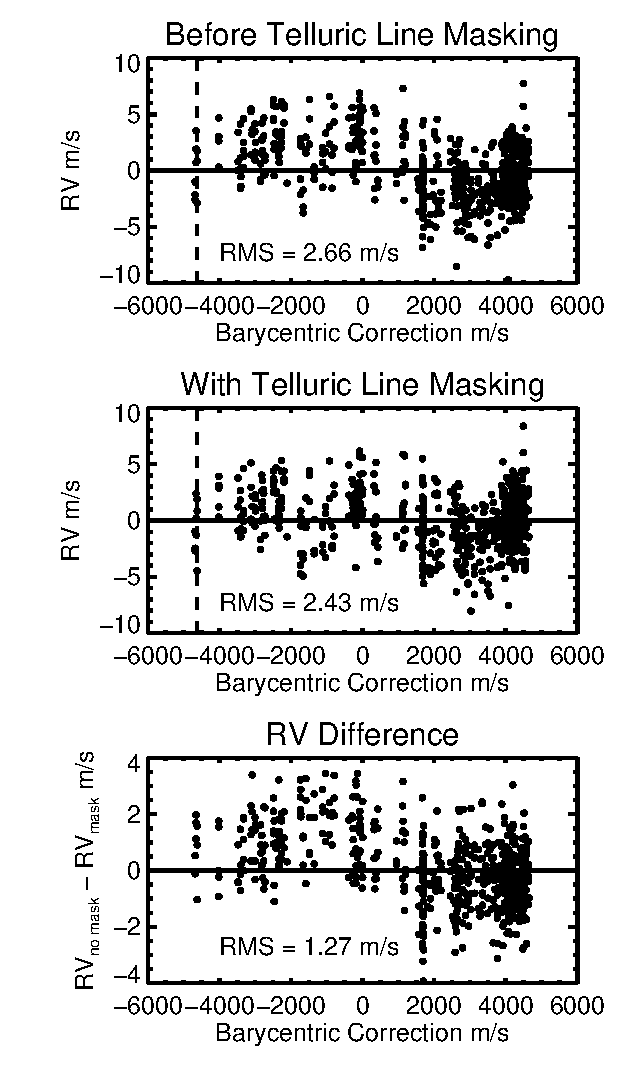
\includegraphics[scale=0.6]{telluric}
    % ~/ExoPlanet-2010-2011/Keck_diagnosis/plots_general/basic_rv/
    % created by basic_rv.pro
    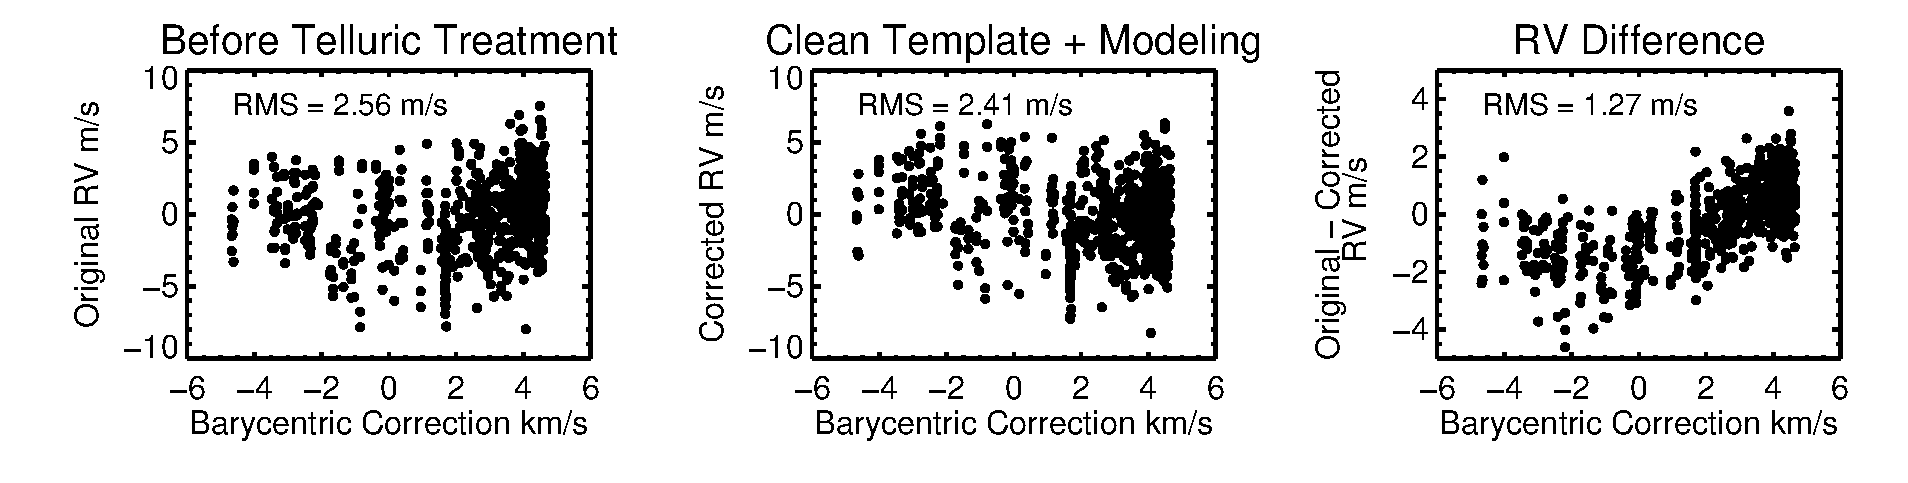
\includegraphics[width=\textwidth]{185144_BC_RV_rj172_4panel}
  \end{center}
  \vspace{-25pt}  
  \caption{Measured precise radial velocities of a standard star
    observed with \keck\ as a function of barycentric correction
    (i.e.~Earth's radial velocity away from the target). Our
    treatment of telluric lines has successfully removed over
    1~\mps\ systematic noise even for this particularly challenging
    stellar template (panel 3; note the change in scale on
    y-axis).} 
  \vspace{-8pt}  
  \label{fig:tell}
\end{figure}


We have also applied our code to a couple more test targets at Keck,
and we are confident that, with telluric-free templates and full
incorporation of telluric lines in the forward-modeling process, we
will be able improve the RV precision and accuracy for many targets at
Keck, especially the stars which have low-mass, low-RV amplitude
planets, such as some of the \kepler\ targets.

Here is a more detailed description of the progress, including ongoing work:

For (a): Stellar spectral templates are derived based on on-sky
observations of the target star without an iodine cell and thus is
also subject to telluric contamination. We have created a pipeline for
producing telluric-free stellar template for Keck (also adaptable for
other instruments). Using the telluric simulation package TERRASPEC
(written by Chad Bender, Penn State, based on the HITRAN molecular
line database; \citealt{hitran2012}), we are able to determine the
oxygen and water column densities based on the red portion of the
spectrum near 7000\AA\ and construct telluric line model for the bluer
iodine region of the spectra. Then for each step in the process of
template creation, we are able to model the telluric lines and
therefore remove it form the end product.

We are now collaborating with the CHIRON group at Yale (Debra Fischer
and Matt Giguere) to provide them with a telluric-free $\tau$ Ceti
template, to enhance the RV accuracy and precision on this important
RV standard star for better understanding of stellar activity induced
RV signal. We are also collaborating with John A.\ Johnson's group at
Harvard to produce an even more superior stellar template which is
derived based on many star$+$iodine observations.

For (b): For the star$+$iodine observations (the RV observations), we
have implemented basic telluric line model plug-in function in our RV
code as a first step, where the water column density would be a fixed
value for all observations. We are constructing the module which would
fit for the water column density for each observation and construct
different telluric models. This would be the final step to fully
modeling the telluric lines in RV observations, and thus provide the
maximal capability of removing the biases within the frame of our
current RV code (for work beyond this, see Section~\ref{sec:newrv}).


%---------------------------------------------------------------------------------------
\vspace{-10pt}
\subsection{Evidence for Changes of Iodine Calibration Cells and Solutions}\label{sec:fts}
\vspace{-5pt}


\begin{wrapfigure}{r}{0.5\textwidth}
  \vspace{-35pt}
  \begin{center}
    % cp /Volumes/RAID/rv/TS12/match_fts/figure/het70_comp.eps ./
    % created by plotcomp.pro
    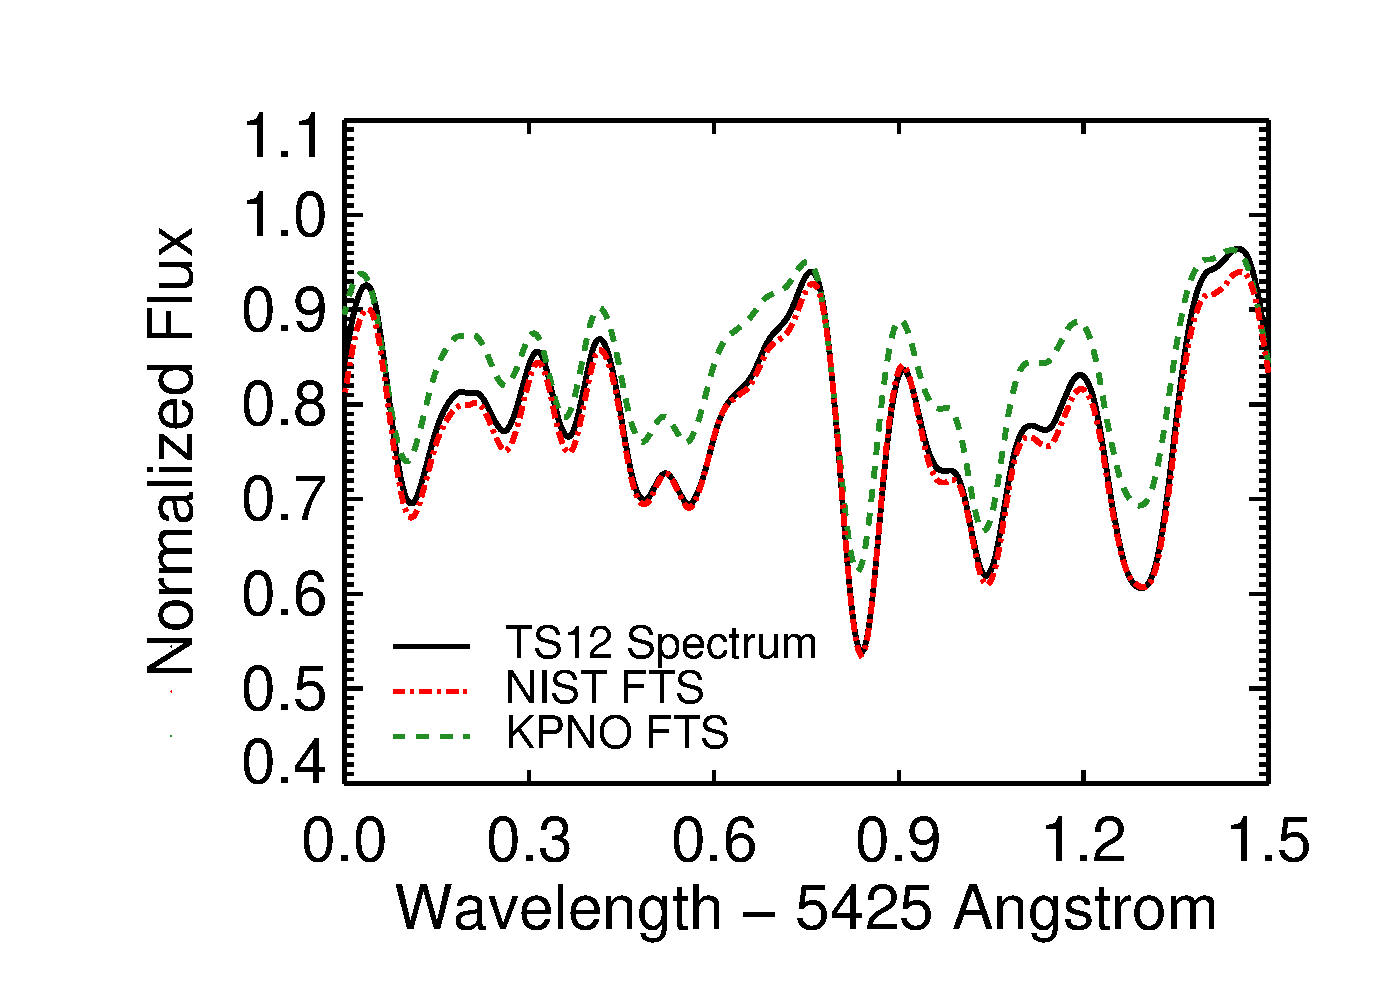
\includegraphics[width=0.5\textwidth]{het70_comp}
  \end{center}
  \vspace{-25pt}  
  \caption{TS12 spectrum vs.\ NIST FTS vs.\ KPNO FTS for the HET/HRS
    iodine cell at 70$\degree$C, all convolved down to a resolution of
    $R=60,000$ (typical RV observation resolution) for comparison
    purposes.}
  \vspace{-8pt}  
  \label{fig:fts}
\end{wrapfigure}


A ``ground truth" iodine atlas is crucial for the precise iodine
radial velocimetry. It is used for modeling the observed iodine lines
in the stellar$+$iodine RV observation to anchor the absolute
wavelengths and the spectrograph response function. Such a ``ground
truth" atlas is normally obtained through a Fourier Transform
Spectrometer (FTS). Our previous work has revealed potential problems
with FTS atlases, and in our original proposal, we promised to use the
TS12 arm of the Tull spectrograph at McDonald Observatory to validate
the qualities of the FTS iodine atlases for HET/HRS, MINERVA, and the
McDonald 2.7m.

In October 2014, the TS12 observations were successfully carried
out. All data are reduced and we have made comparisons between the
TS12 spectra and FTS scans. For the 2.7m cell, its TS12 spectrum
matches very well to its FTS atlas, again (together with the 2.1m cell
data from 2013) proving that TS12 is an appropriate tool for
validating FTS atlases. The TS12 spectra for the MINERVA cell is also
ready, and right now we are waiting for the FTS expert on our team to
reduce the MINERVA FTS data for comparison, which is expected to be
done before June (first light of the proto-type MINERVA spectrograph).

Finally, for the HET/HRS iodine cell, we have taken its TS12 spectra
at three different temperatures (50, 60, and 70$\degree$C; the RV
working temperature for the cell is 70$\degree$C). Our main findings
(both are first-time discoveries for iodine RV work) are as follows:

(a) Temperature change (5--10$\degree$C) in iodine cell matters: The
long suspected temperature-induced iodine spectrum change was finally
confirmed, which is seen very visibly among the TS12 spectra taken at
three different temperatures. Based on our NIST FTS atlases taken at
two different temperatures, temperature change on the order of
10$\degree$C should not induce visible line changes. However, we
suspected issues with temperature control and data calibration with
the NIST atlases, and the TS12 spectra confirmed our suspicion and
proved that temperature on the order of even 5$\degree$C would have
manifested as significant line changes (for precise RV purposes).

(b) The HET/HRS cell very likely has changed over time: The TS12
spectra match better with the more recent but potentially problematic
NIST FTS atlas, which had worse $\chi^2_\nu$ fit than the old KPNO
atlas. This is completely unexpected and suggests that: the NIST atlas
was perhaps taken at the correct temperature (i.e.\ the KPNO atlas was
at a lower and wrong temperature) but the worse fit was caused by
calibration errors in the atlas; and/or the temperature or optical
depth of the cell changes over the course of 20 years, and hence the
differences between these three spectra (Figure~\ref{fig:fts}); and
further more, it is possible that the temperature/optical depth of the
cell changes on a much shorter scale during the observing seasons, and
most of the time it stays at a temperature/optical depth that is
similar to the one when the KPNO atlas was taken (e.g.\ actually at a
lower temperature though thought to be at 70$\degree$C).

To answer these questions and to actually resolve the issue of a
changing cell, we have found a possible third venue that might provide
reliable, ultra-high resolution, and wavelength calibrated iodine
atlas -- a theoretical code that computes iodine transmission spectrum
(at any specified temperature) based on both physics and empirical
calibrations (IodineSpec5; \citealt{iodinespec5}). We have
successfully installed and learned the code, and properly translated
the code output into practical astrophysical units and to account for
optical depth differences. We are now using the code to diagnose the
HET/HRS cell to study whether the cell temperature or optical depth
changes (as reflected by actual HET/HRS observations instead of
FTS/TS12 atlas observations), and to explore the possibility of using
the theoretical output as the new ``ground-truth" atlas.


%---------------------------------------------------------------------------------------
\vspace{-10pt}
\subsection{A Better Instrumental Profile Model for Fiber-Fed Spectrographs}\label{sec:ip}
\vspace{-5pt}

One limiting factor for the current RV precision of \hrs\ is the
modeling of its instrumental profile (IP, or the spectrograph response
function or spectral PSF). In our original proposal, we promised to
look for a better IP for \hrs, as a test case for future fiber-fed
precise RV spectrographs, such as the upcoming MINERVA and the future
fiber-fed Keck/HIRES.

The old IP model for \hrs\ is the very versatile, orthogonal,
11-parameter Gauss-Hermite polynomials (GH). However, through our
analyses using calibration frames in Fourier space, we have found that
although GH is probably sufficient to describe the \hrs\ IP, because
of its ultra flexibility and multi-parameters, it deeply complicates
the $\chi^2$ space and very often hinders the fitter from finding the
true minimal (to address the issue with the fitter, see next section
and future plans). A simpler IP is therefore in great desire.

We have found a better IP function for \hrs, the modified Moffat function:
\begin{equation}
[1+(x/\theta)^2]^{-\beta\cdot(x/\delta)^2}
\end{equation} 
It is called the ``modified" Moffat function because the original
Moffat function does not have the $(x/\delta)^2$ term. We added this
term to add flexibility at the wings to enable change of characteristic
IP width while preserving wing profile. Figure~\ref{fig:ip}
illustrates the results: black line is the $\chi^2_\nu$ distribution
for fitting spectral chunks in an observation with GH IP; red line is
for modified Moffat IP; and dashed red is for fixing the IP in the
shape of a thorium line (proving that thorium line is a good proxy for
IP). This 3-parameter function fits the \hrs\ data almost equally
well, and it fits very well to the observed thorium line
(Figure~\ref{fig:ip} inset, dots are observed thorium line).


\begin{wrapfigure}{l}{0.55\textwidth}
  \vspace{-35pt}
  \begin{center}
    %~/ExoPlanet-2010-2011/HET-HRS-IP/06-line_through_dots/thar_vs_moffat.eps
    % made by thar.pro
    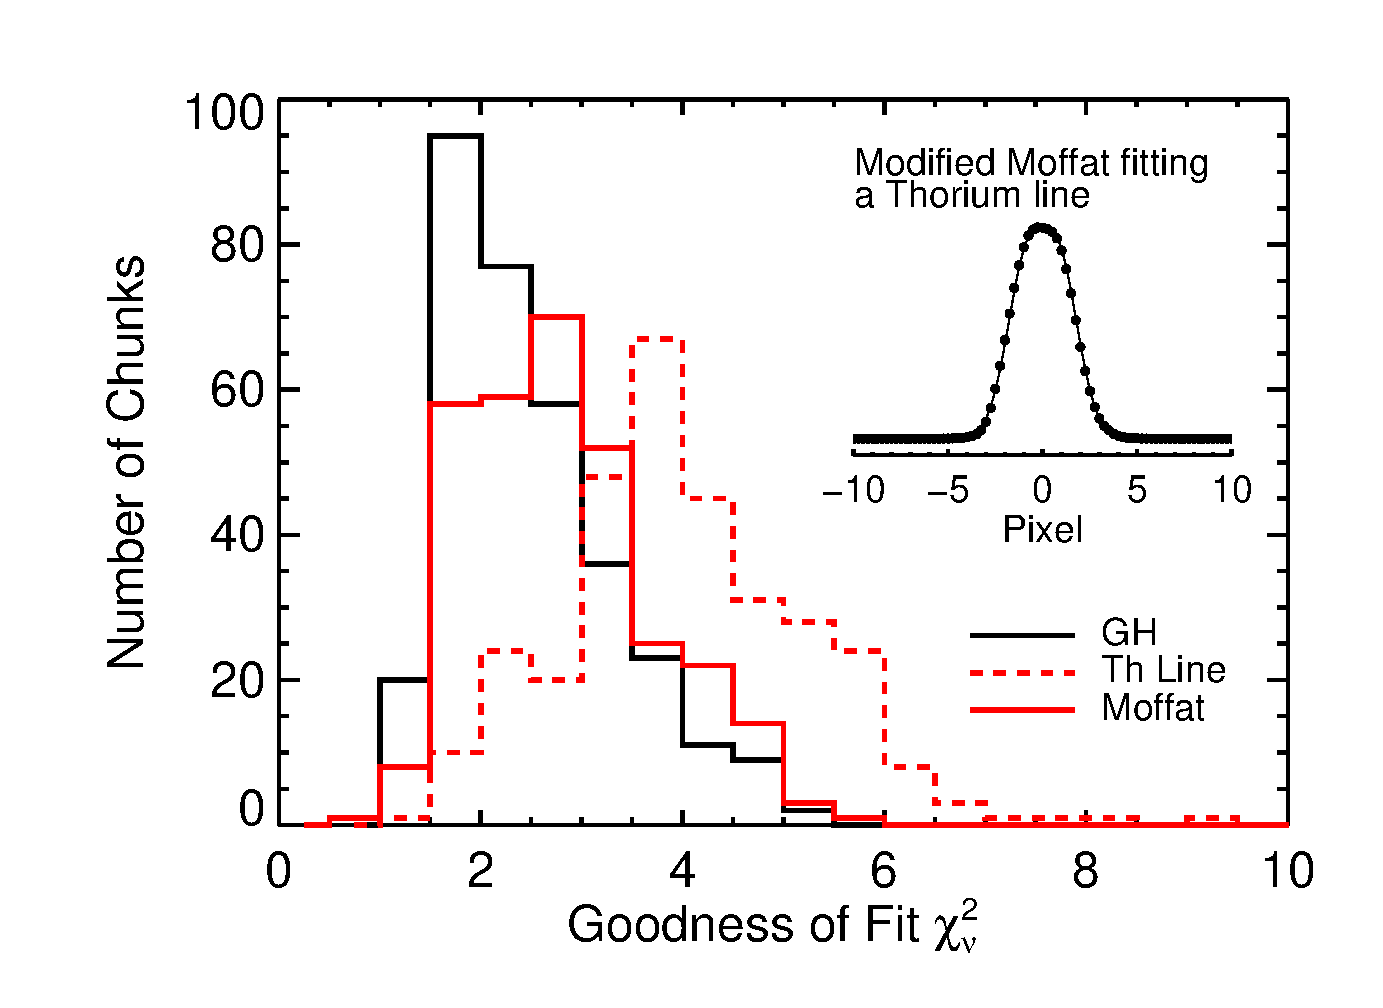
\includegraphics[width=0.52\textwidth]{thar_vs_moffat}
  \end{center}
  \vspace{-25pt}  
  \caption{Histogram of goodness of fit, $\chi_\nu^2$, values for
    spectral chunks of a calibration frame. The modified Moffat
    function (red) performs almost equally well while having only 3
    parameters, compared with the complicated 11-parameter GH function
    (black solid).} 
  \vspace{-8pt}  
  \label{fig:ip}
\end{wrapfigure}


This modified Moffat function is potentially applicable to other
fiber-fed instruments, since these instruments tend to have IPs with
the same characteristic flat top and sharp wings.

Our ongoing work includes: adding small perturbation terms to the
modified Moffat IP to account for IP asymmetry and subtle wings due to
scattered light etc.; disentangling the effects of a bad IP model and
bad iodine atlas (as described in previous section); and other tests
with the aim to bring $\chi^2_\nu$ for fitting \hrs\ data to $\sim 1$,
which is what is achieved at Keck and enabled $\sim 1$ \mps\ RV
precision.



%---------------------------------------------------------------------------------------
\vspace{-10pt}
\subsection{Building the Next-Generation Data Analysis Tools for Future RV Surveys}\label{sec:newrv}
\vspace{-5pt}

The work described in the previous sections is all done with the
California Planet Search Consortium Doppler code, which is a legacy
code in IDL primarily written by John A.\ Johnson but with legacy
parts that date back to the work of Marcy \& Butler as early as
1989. It is proven to be able to produce RVs at $\sim 1$
\mps\ precision with Keck data, and is behind the discoveries and
characterization of numerous exoplanets, including the first
Earth-mass Earth-radius planet Kepler-78b \citep{howard2013,pepe2013}.

Yet, this great legacy code has many drawbacks: It is based on a
simple home-constructed Levenberg–-Marquardt least $\chi^2$ fitter
(LM fitter) which has high requirement on initial guesses for
parameters and is terribly inefficient and inadequate in exploring the
$\chi^2$ space. It also has many legacy house keeping parts and
complicated structures that makes it hard to upgrade, adopt for other
instruments, and add new modules and functions.

We have set out to write a new RV code that is built in {\it Python}.
The new code carries on the valuable successful parts of the CPS code
over, and more importantly, built to be highly modular and thus will
be easy to adopt for other instruments or to plug in modern
numerical and statistical tools.

We have completed the structural design and built the core part of the
code, where it fits one spectral chunk using any designated maximum
likelihood style fitter (e.g.\ a better LM fitter, which yield a
smaller $\chi^2_\nu$ value when testing with Keck spectral chunks). We
plan to make it fully functional for the commissioning of MINERVA in
Summer 2015 (see Section~3 for future plans to implement more
advanced tools).

Currently there is a large cry in the RV community for a public,
high-precision RV code which would allow better transparency and cross
checking of results. We have made our code publicly available through
{\tt gitHub}, and we plan to document the methods in peer-reviewed
literature once the code is ready to be released for the greater
community.


%%%%%%%%%%%%%%%%%%%%%%%%%%%%%%%%%%%%%%%%%%%%%%%%%%%%%%%%%%%%%%%%%%%%%%%%%%%%%%%%%%%%%%%%%
\vspace{-10pt}
\section{Future Plans}
\vspace{-5pt}

We have briefly touched on some of the future plans for the next
funding cycle in the sections above. Here to summarize and elaborate:

1.\ After finishing implementing forward-modeling of telluric lines in
the RV code, we plan to re-run RV analyses for important targets such
as the \kepler\ systems with low-mass planets (e.g.\ the
\citealt{Marcy2014} targets), and dynamically interesting systems such
as 55 Cancri, GJ 876, $\upsilon$ Andromedae, and GJ 581 (as promised
in the original proposal). Publication on the telluric line treatments
and any interesting science outcome from the re-analyses is among our
top priorities.

2.\ If we can successfully improve the fitting with \hrs\ data with
better iodine atlas and better IP modeling, we plan to re-run systems
with low-mass planets and systems that are not among the Keck target
list or not as frequently observed, to see if a higher precision will
bring discoveries of more planets and better characterization of
existing ones. Again, publication of the work on iodine atlas and any
science outcome from the re-analyses is our top priority.

3.\ We plan to implement modern packages into our new RV code for more
statistically robust estimates of RVs. In particular, we plan to go
Bayesian by using the MCMC package, {\tt emcee}, by \cite{emcee},
which will essentially eliminate the issues of unstable/inefficient
fitter, requirements on initial guesses, and unreliable/ambiguous
error bars. Adopting Bayesian methods will also redefine and largely
improve the wavelength-dependent statistical weighting process (which
we are also currently exploring within the old code frame, in
collaboration with Ben Nelson at PSU/Northwestern; as promised in the original
proposal). To address the issue of stellar template uncertainties or
any other persisting systematic effects in the spectra
(e.g.\ residuals left after modeling out the telluric lines), we plan
to implement the {\tt StarFish} package by \cite{starfish}, which uses
Gaussian processes to account for systematics in spectral
modeling. These model packages will bring the Doppler analysis to the
next level, and produce a truly modern code for modern RV surveys.



%%%%%%%%%%%%%%%%%%%%%%%%%%%%%%%%%%%%%%%%%%%%%%%%%%%%%%%%%%%%%%%%%%%%%%%%%%%%%%%%%%%%%%%%%
%\newpage
%\addcontentsline{toc}{section}{References}
\vspace{-3pt}
\bibliographystyle{apj}	% (uses file "xxx.bst")
%\begin{multicols}{2}
{\small % smaller fonts for references
%{\footnotesize
\bibliography{references} }
%\end{multicols}


%%%%%%%%%%%%%%%%%%%%%%%%%%%%%%%%%%%%%%%%%%%%%%%%%%%%%%%%%%%%%%%%%%%%%%%%%%%%%%%%%%%%%%%%%

\end{document}
